% Kompilováno pomocí XeLaTeXu (TeXLive 2021) na Fedoře 36

\documentclass{fkssolpub}

\usepackage[czech]{babel}
\usepackage{fontspec}

\usepackage{hyperref}
\usepackage{graphicx}

\usepackage{biblatex}
\addbibresource{Bibliografie.bib}

\author{Ondřej Sedláček}
\school{Gymnázium Oty Pavla} 
\series{2}
\problem{4} 

\begin{document} 

\section{Problém 4 -- Využítí hledání extrémů a monotonií}

Protože hledání extrémů a monotonií je jedno ze základů diferenciálního
počtu, podobně jako diferenciální počet se využívá v mnoha oborech.
Zde si ukážeme využití v několika z nich a využití v několika příkladech
uvedených v zadání.

\subsection{Ekonomie}

Protože při dostatečné abstrakci jsme schopni příjem a náklady vyjádřit
jako funkci s jednou neznámou, můžeme samozřejmě hledat její extrémy a 
tím maximalizovat zisk či maximalizovat příjem.

Nejdříve věnujeme pozornost maximalizaci příjmu. Protože pro ziskovou
funkci $PR(q)$, nákladovou funkci $C(q)$ a příjmovou funkci $R(q)$,
kde $q$ je množství prodaného zboží, platí \cite{zahradnickova_ekonomicke_2009}
\cite{mazurek_matematika_2013}:

\[
  PR(q) = R(q) - C(q)
\]

Pak platí:

\[
  PR'(q) = R'(q) - C'(q) = 0
\]
\[
  R'(q) = C'(q)
\]

A poněvadž mezní příjem $MR(q) = R'(q)$ a mezní náklady $MC(q) = C'(q)$,
odvodili jsme za pomoci derivací jedno z ekonomických pravidel 
\cite{noauthor_slovnicek_nodate} \cite{mazurek_matematika_2013}, 
a to že při maximalizaci výroby se mezní příjmy rovnají mezním nákladům. 

Pokud však místo výrobků prodáváme třeba lístky nebo licence, mezní
náklady budou nulové. Ale zase samozřejmě se může měnit poptávka se
změnou ceny, tudíž při maximalizaci příjmu se pokoušíme zjistit takovou
cenu, kdy bude příjem nejvyšší. V tomto případě bude příjem roven
součinu ceny a množství. \cite{zahradnickova_ekonomicke_2009} 
\cite{mazurek_matematika_2013}

Oboje si teď ukážeme na příkladech:

\textbf{Příklad 1.} 
\textit{Společnost vyrábějící mluvící robůtky na kolečkách pro děti 
má nákladovou funkci $C(q) = q^2 + 10q + 100$ příjmovou funkci
$R(q) = 900q$. Určete množství $q$, při kterým bude zisk maximalizován.}

\textbf{Řešení.}

Víme, že extrémy se nachází v bodech, kdy $R'(q) = C'(q)$. Tudíž musíme
jako první zjistit derivace.

\[
  R'(q) = 900 \cdot (q)' = 900
\]

\[
  C'(q) = (q^2)' + (10q)' + (100)' = 2q + 10
\]

To, když dosadíme, vyjde nám:

\[
  R'(q) = C'(q)
\]
\[
  900 = 2q + 10
\]
\[
  890 = 2q
\]
\[
  q = 445
\]

Teď si ověříme, že to není minimum. Protože v intervalu 
$(-\infty; 445 \rangle$ zisková funkce $\pi(q) = R(q) - C(q)$ roste a 
v intervalu $\langle 445; +\infty)$ klesá, musí se jednat o maximum. 
Proto výsledek bude $q = 445$.

\textbf{Příklad 2.}
\textit{Cena licence softwaru na úpravu fotografií je definována
v eurech jako $p(q) = 200 - 0,01q$. Určete množství $q$, při kterým bude 
příjem $R(q)$ maximalizován.}

\textbf{Řešení.}

Zde bude příjem roven $R(q) = p(q) \cdot q$. Proto jako první dosadíme
funkci $p(q)$ do $R(q)$ a pak zderivujeme.

\[
  R(q) = p(q) \cdot q = (200 - 0,01q) \cdot q = -0,01q^2 + 200q
\]
\[
  R'(q) = (-0,01q^2)' + (200q)' = -0,01 \cdot 2q + 200 = -0,02q + 200
\]

Následně najdeme extrémy:

\[
  R'(q) = -0,02q + 200 = 0
\]
\[
  200 = 0,02q
\]
\[
  q = 10000
\]

Zde příjmová funkce v intervalu $(-\infty; 10000 \rangle$ roste a v 
intervalu $\langle 10000; +\infty$ klesá, tudíž se jedná o maximum. 
Proto $q = 10000$.

\subsection{Umělá inteligence}

Další odvětví, kde se využívá znalostí matematické analýzy o hledání
extrémů, je umělá inteligence. Přesněji nahlédneme do fungování strojového
učení a ukážeme si, kde se hledání extrémů v ní využívá.

\begin{figure}[h!]
  \centering
  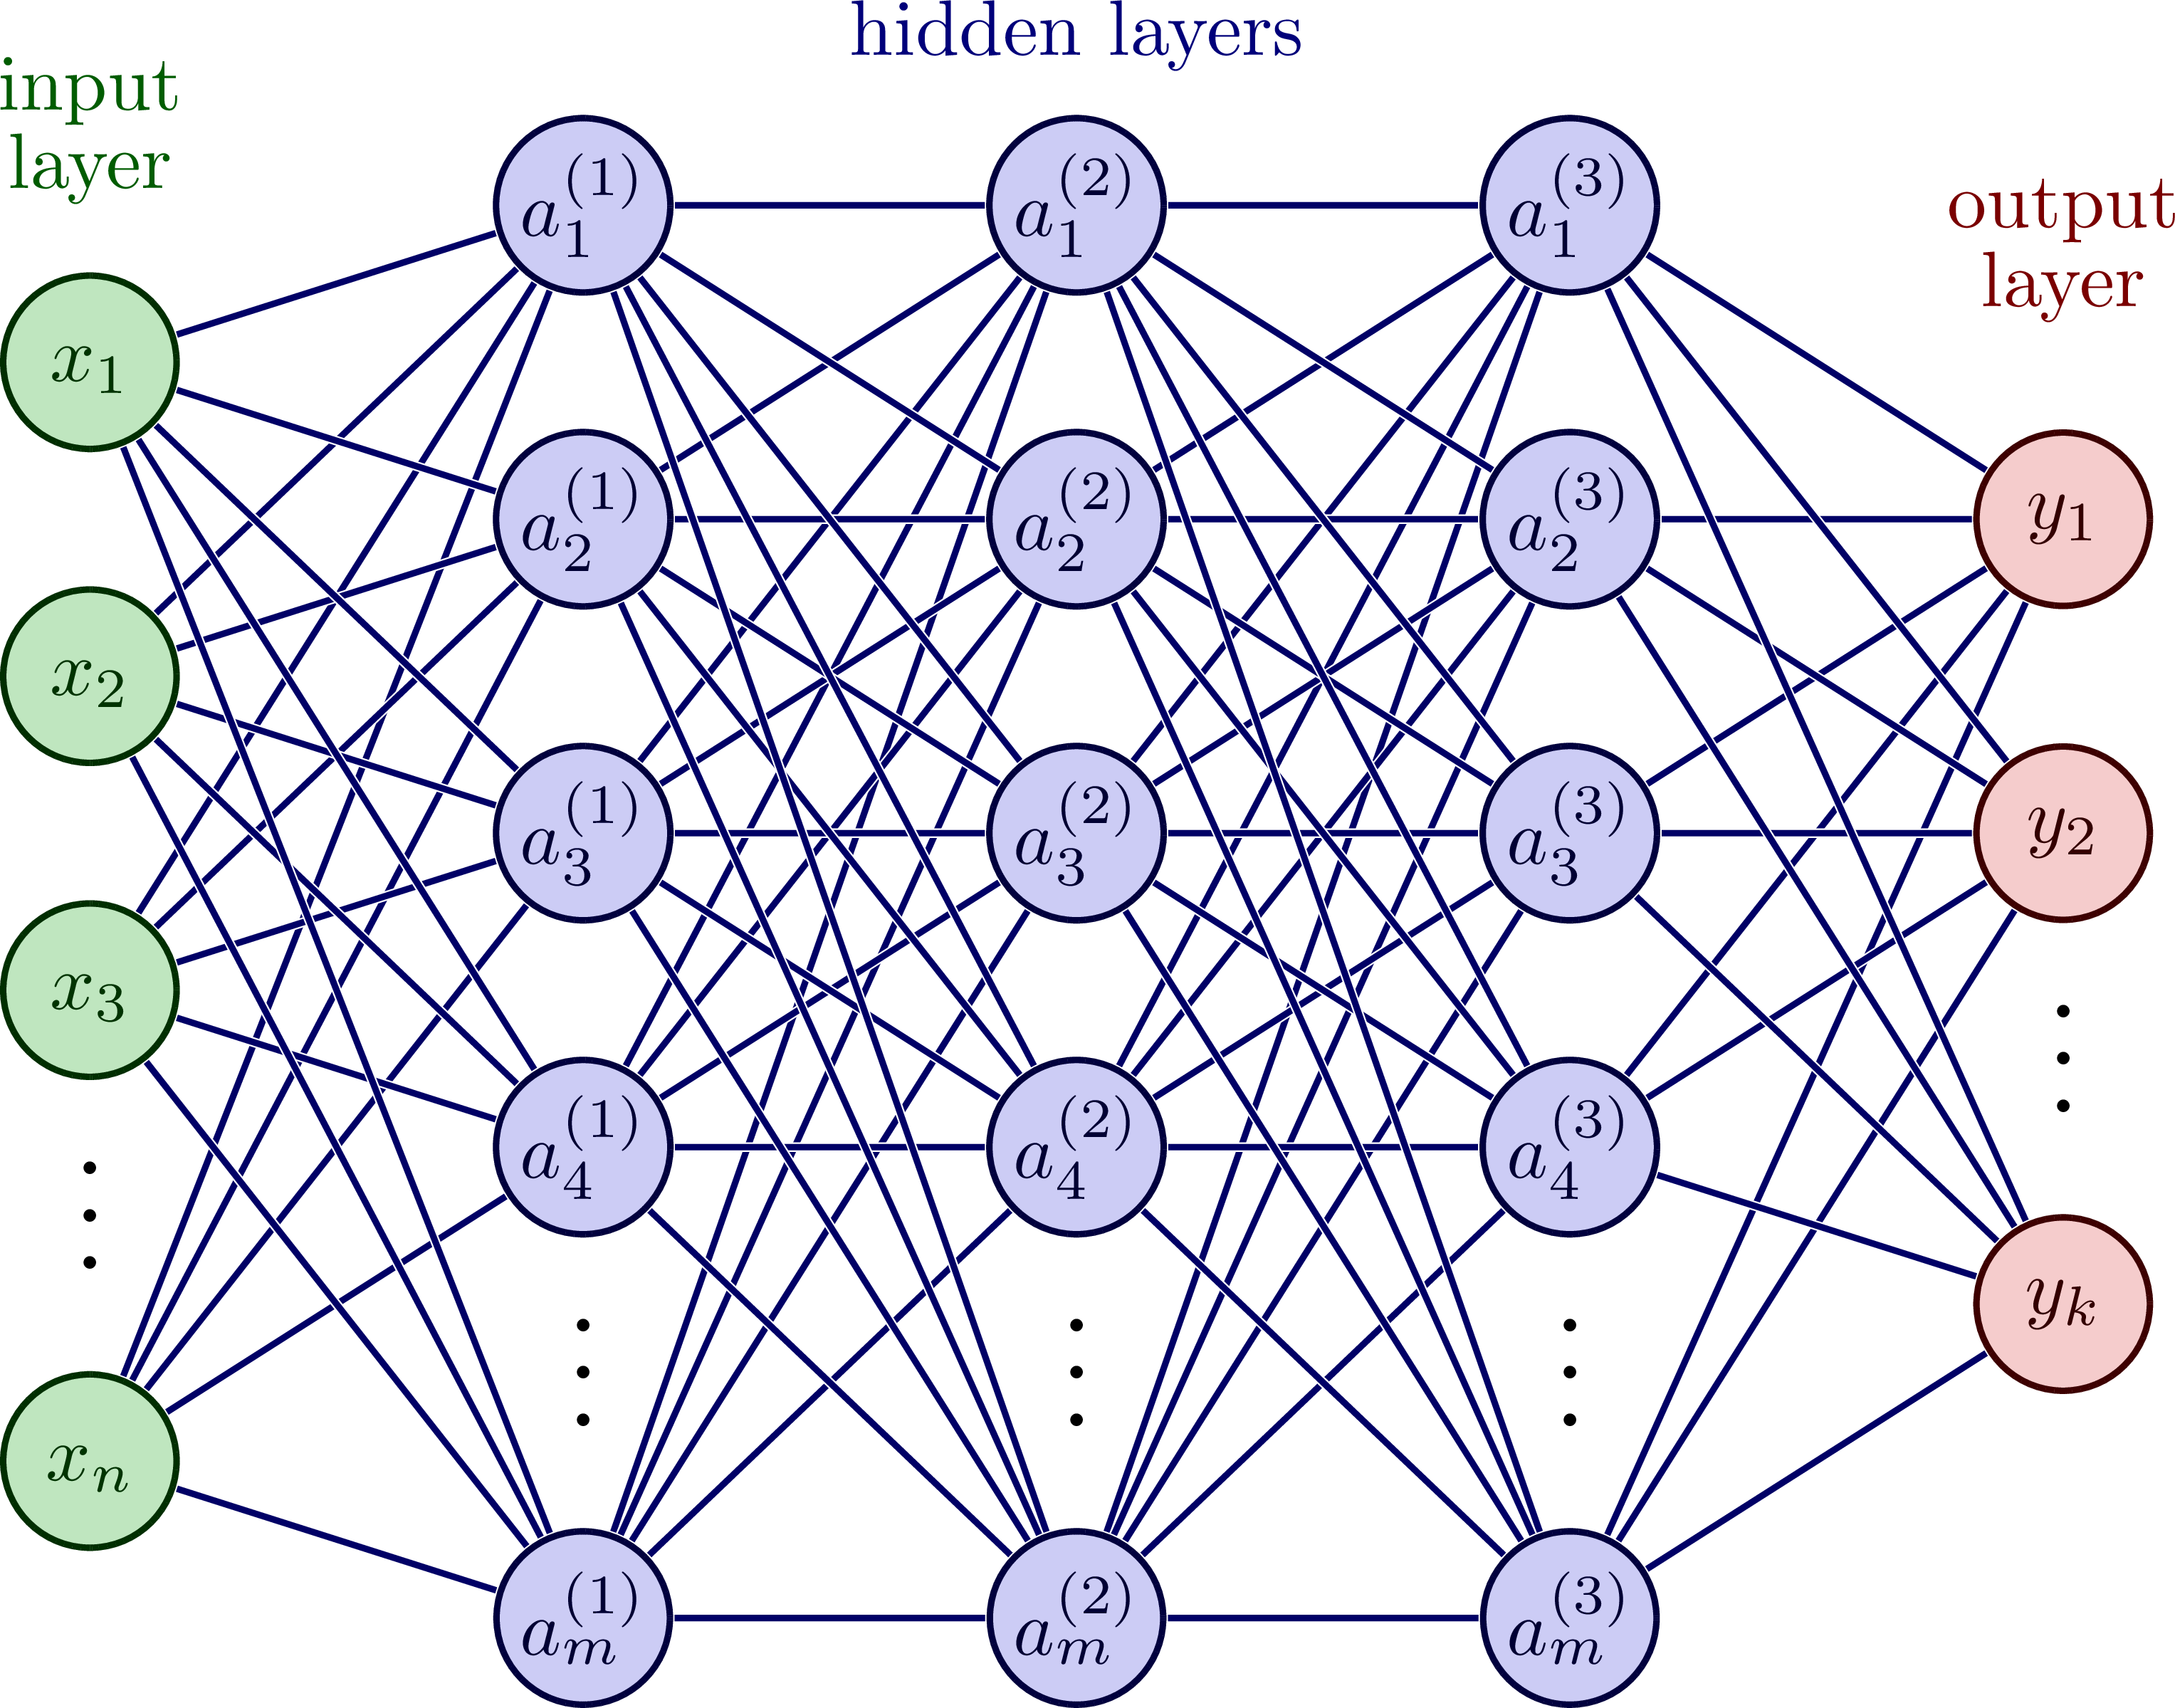
\includegraphics[width=\textwidth]{neural_networks.png}
  \caption{
    Příklad neuronové sítě (zdroj: 
    \url{https://tikz.net/wp-content/uploads/2021/12/neural_networks-004.png})
  }
  \label{fig:network}
\end{figure}

Nejdříve si však stručně vysvětlíme fungování jeden ze základních
typů neuronových sítí, kde se tento algoritmus používá. Na obrázku
vidíte, že jednotlivé neurony jsou uspořádané do vrstev -- vstupní vrstvy,
skrytých vrstev a výstupní vrstvy.  Každý neuron je spojený s každým 
neuronem v předchozí vrstvě, každý ten spoj má určitou váhu a každý neuron 
má určitou konstantu "bias". Tyto hodnoty jsou zásadní
pro to, aby neuronová síť vracela správný výsledek. Avšak nejdříve musíme
tyhlety hodnoty zjistit. \cite{3blue1brown_but_2017}

Na začátku se tyto konstanty určí náhodně. Pak se opakuje následující 
postup. Nejdříve se dosadí vstupní hodnoty
do vstupní vrstvy.Pak se určujou hodnoty dalších neuronů tak, že se vypočítá
vážená suma hodnot neuronů v předchozí vrstvě, od nich se odečte "bias" a to
celé se pak vloží do funkce sigmoid, což je logickická funkce s hodnotovým
oborem $(0;1)$. \cite{noauthor_sigmoid_2022} \cite{3blue1brown_but_2017}
Jakmile jsou vypočteny hodnoty neuronů ve
výstupní vrstvě, vypočítá se hodnota chybové funkce $C$ jako suma čtverců 
odchylek od správného výsledku. Tato funkce má váhy a biasy jako proměnné 
a vstup jako parametr. A protože chceme, aby byla chyba co nejmenší, 
musíme najít její minimum. Ale poněvadž máme až příliš mnoho proměnných, 
můžeme jedině najít sklon dané funkce a pak se posunout směrem k minimu.
\cite{3blue1brown_gradient_2017}

Tomuto postupu se říká gradientní sestup, protože najde gradient v daném
bodě a pak jde opačným směrem proti němu. Na tomto postupu je založený
důležitý algoritmus strojového učení algoritmus zpětného šíření chyby 
(anglicky backpropagation) založený -- podle hodnoty chybové funkce postupně 
vrstvu po vrstvě mění hodnoty jednotlivých konstant. Bohužel lze tímto postupem 
najít jen lokální minimum, což ale je často postačující. 
\cite{3blue1brown_gradient_2017}

\newpage

\subsection{Statistika}

Ještě chci zmínit jednu centrální metodu matematické statistiky a to metodu
maximální věrohodnosti. 

Předpokládejme, že máme určitý statistický soubor dat, třeba EQ obyvatel, 
a chceme být schopni odhadnou, jak častí budou obyvatelé s EQ,
který neměj nikdo v daném vzorku obyvatelstva. Pak budeme muset vybrat
určité rozdělení, které bude nejlépe odpovídat danému souboru. Mezi ně
patří normálové (jejíž tvar je Gaussova křivka, pro tento typ dat
nejpravděpodobnější), exponenciální či gama rozdělení. Avšak funkce
těchto rozdělení mají parametry, které mění tvar daného rozdělení. 
Zde pak přichází na radu zmiňovaná metoda. 
\cite{statquest_maximum_2017}

Jejím cílem je najít takový parametr $\theta$, pro
kterou je pravděpodobnost, že pozorované hodnoty pocházejí z předpokládaného
rozdělení, maximální. \cite{noauthor_matematicka_nodate} 
\cite{noauthor_metoda_2022}

Nechť funkce sdružené hustoty $f(x_1, ..., x_n|\theta)$ je definován jako:

\[
  f(x_1, ..., x_n|\theta) = \prod \limits_{i=1}^n f(x_i|\theta)
\]

Kde $f(x|\theta)$ je funkce rozdělení. Pak se parametr $\theta$ určuje u 
spojitého rozdělení hledáním extrému za pomocí derivace věrnostní funkce 
$\mathcal{L}(\theta|x_1, ..., x_n)$, která je s funkcí združené hustoty
totožná až na prohozené proměnné a parametry. \cite{noauthor_matematicka_nodate}
\cite{noauthor_metoda_2022}

Bohužel se při výpočtu pracuje s nekonečnými sumami a produkty, což
by dle mého názoru přesáhl rámec tohoto textu. Proto pokud máte zájem o
nějaký příklad, jeden můžete najít na české Wikipedii 
(\url{https://cs.wikipedia.org/wiki/Metoda_maxim\%C3\%A1ln\%C3\%AD_v\%C4\%9Brohodnosti}).


\subsection{Užití na příkladech ze zadání}

Jako poslední tu ukáži využití hledání extrémů a monotonií na
dvou příkladech ze zadání pro ty, kteří tento problém neřešili nebo chtějí
vidět řešení někoho jiného, přesněji na hledání vrcholu paraboly 
a vrhu šikmého.

\subsubsection{Hledání vrcholu paraboly}

Pro hledání vrcholu paraboly ani nemusíme použít derivace, pokud známe
vrcholový tvar kvadratických funkcí \cite{odvarko_matematika_1994}:

\[
  f(x) = a\left(x + \frac{b}{2a}\right)^2 + \left(c - \frac{b^2}{4a}\right)
\]

A víme, že na ose $x$ se bude vrchol nacházet v $x = -\frac{b}{2a}$. Ale
pokud chceme použít metody matematické analýzy, pak stačí kvadratickou
funkci zderivovat, pak najít, kdy se derivace protíná s osou $x$, a 
ověřit si, že se jedná o globální extrém.

\subsubsection{Vrh šikmý}

Další příklad je vrh šikmý. Pro ten budu zanedbávat odpor a jeho 
trajektorie bude začínat v počátku. 

% Nebyl jsem schopný skompilovat obrázek pomocí \includestandalone,
% proto jsem ho skompiloval samostatný a pak převedl do PNG.

\begin{figure}[h!]
  \centering
  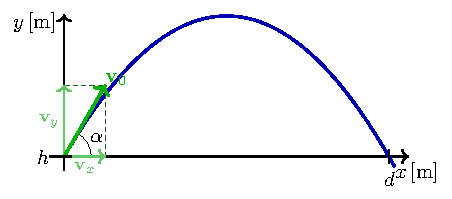
\includegraphics[width=\textwidth]{projectile}
  \caption{Nákres vrhu šikmého (zdroj původního obrázku: 
    \url{https://tikz.net/kinematics_trajectory2/})}
  \label{fig:projectile}
\end{figure}

Protože vrh šikmý je pohyb složený z pohybu rovnoměrného přímočarého
a volného pádu, můžeme jednoduše za pomoci obrázku \ref{fig:projectile} určit
vztah pro $x$ a pro $y$ \cite{realisticky_vrh_nodate}:

\[
  x = v_0 t \cos{\alpha}
\]

\[
  y = v_0 t \sin{\alpha} - \frac{1}{2}g t^2
\]

V těchto rovnicích máme dvě neznámé -- čas $t$ a úhel $\alpha$, tudíž
ty funkce nemůžeme rovnou zderivovat. Avšak času $t$ jsme se schopni
zbavit dosazením z jiného vztahu.

Začneme nejdříve u maximální výšky $y_m$. Protože při dosažení maximální
výšky je okamžitá rychlost $v_y$ nulová, platí:

\[
  v_y = v_0 \sin{\alpha} - g t = 0
\]
\[
  v_0 \sin{\alpha} = gt
\]
\[
  t = \frac{v_0 \sin{\alpha}}{g}
\]

Když dosadíme toto do vztahu pro $y$, dostaneme maximální výšku:

\[
  y_m = v_0 \sin{\alpha} \cdot \frac{v_0 \sin{\alpha}}{g} 
   - \frac{1}{2} g \cdot \left(\frac{v_0 \sin{\alpha}}{g}\right)^2
   = \frac{v_0^2 \sin^2{\alpha}}{g} - \frac{v_0^2 \sin^2{\alpha}}{2g}
   = \frac{v_0^2 \sin^2{\alpha}}{2g}
\]

U dostřelu zase bude platit, že souřadnice $y$ bude nulová, proto bude platit:

\[
  y_d = v_0 t \sin{\alpha} - \frac{1}{2} g t^2 = 0
\]
\[
  v_0 \sin{\alpha} = \frac{gt}{2}
\]
\[
  t = \frac{2 v_0 \sin{\alpha}}{g}
\]

Po dosazení do vztahu pro $x$ získáme dostřel:

\[
  d = v_0 \cos{\alpha} \cdot \frac{2 v_0 \sin{\alpha}}{g}
    = \frac{2 v_0^2 \sin{\alpha} \cos{\alpha}}{g}
\]

Teď už můžeme jak maximální výšku $y_m$, tak dostřel $d$ zderivovat:

\[
  y_m' = \left(\frac{v_0^2 \sin^2{\alpha}}{2g}\right)' = \frac{v_0^2}{2g}
    \cdot (\sin^2{\alpha})' = \frac{v_0^2}{2g} \cdot 2 \sin{\alpha} \cos{\alpha}
    = \frac{v_0^2}{2g} \sin{2 \alpha}
\]
\[
  d' = (\frac{2 v_0^2 \sin{\alpha} \cos{\alpha}}{g})' = \frac{2 v_0^2}{g}
    \cdot (\sin{\alpha} \cos{\alpha}) = \frac{2 v_0^2}{g}
    \cdot (\cos^2{\alpha} - \sin^2{\alpha}) = \frac{2 v_0^2}{g} \cos{2 \alpha}
\]

Protože se derivace každé z nich musí rovnat nule, vyplývá z toho, že
nulové hodnoty pro maximální výšku jsou $0^{\circ}$ a $90^{\circ}$ a pro dostřel
$45^{\circ}$. Když vyřadíme úhel $0^{\circ}$, protože při něm hmotný bod nikam
nedoletí, pak máme řešení.

\subsection{Závěr}
Jak jste si mohli všimnout v naprosté většině případů se hledání extrémů
a monotonií pojí s optimalizací. To se také ukazuje na 
mnoha slovních úlohách, mezi které patří například tato 
\cite{jelinkova_aplikacni_2013}:

\textit{"Majitel restaurace chce oplotit svůj obdélníkový pozemek přimykající se jednou stranou
k budově restaurace. Obsah pozemku je roven 800 m$^2$. Jaký by měl pozemek mít rozměry,
aby majitele oplocení vyšlo co nejlevněji, tj. aby délka plotu byla co nejmenší?"}

Po přečtení jsem si celkem jistý, že tuto úlohu budete schopni vyřešit,
jako jsem si jistý, že pokud jste o smysluplném využití hledání extrémů
a monotonií pochybovali, už o tom nepochybujete.

\printbibliography[title=Zdroje]

\end{document}
